\subsection{Sampling-scheme ablation}
We evaluated two sampling schedules at 10, 20, 40 and 80 frames: autoregressive stabilization and full-sequence chunk-two sampling. Each condition contains eight videos at seed zero. Late-window LPIPS for autoregressive sampling is 0.1433, 0.1248, 0.1157 and 0.1366; for full-sequence sampling it is 0.1641, 0.1337, 0.1655 and 0.1421. Neither schedule shows a monotonic increase across horizons. At $8\times$, full-sequence MSE is lower (0.01304 versus 0.01780), while LPIPS is slightly higher (0.1421 versus 0.1366). These metrics measure temporal change, so smaller values alone do not imply better generation. At $4\times$ both changes are larger for full-sequence sampling. There is no consistent quality winner in this small sample.

Full-sequence sampling takes 29.8--387.4 seconds per video versus 55.0--766.3 for autoregressive sampling, a measured speedup of 1.85--1.98 across conditions. Timing includes startup and logging. Video repeats were omitted because the initial eight completed runs exceeded the predefined 1.5 GPU-hour threshold. Error bars therefore describe variation across eight videos, not seed uncertainty or confidence intervals. Horizon-dependent clip selection confounds cross-horizon comparisons. At $1\times$, early and late windows coincide. Qualitative sampled-frame review found no gross collapse, but did reveal geometry and object discontinuities in both schedules.

\IfFileExists{figures/ablation_curves.pdf}{
\begin{figure}[ht]
\centering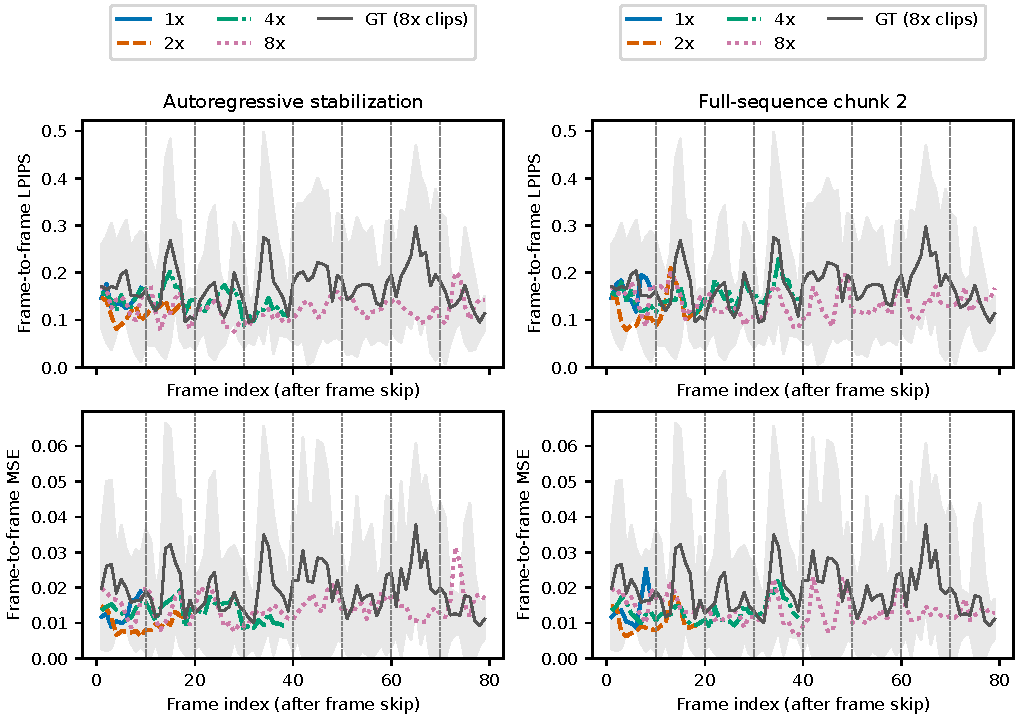
\includegraphics[width=\linewidth]{figures/ablation_curves.pdf}
\caption{Our sampling-scheme ablation: LPIPS (top) and MSE (bottom) between consecutive frames. Left: autoregressive stabilization. Right: full-sequence chunk-two sampling. Shading shows valid ground-truth mean plus or minus video standard deviation; dashed vertical lines mark ten-frame horizon boundaries.}
\end{figure}}{}
\IfFileExists{figures/ablation_summary.pdf}{
\begin{figure}[ht]
\centering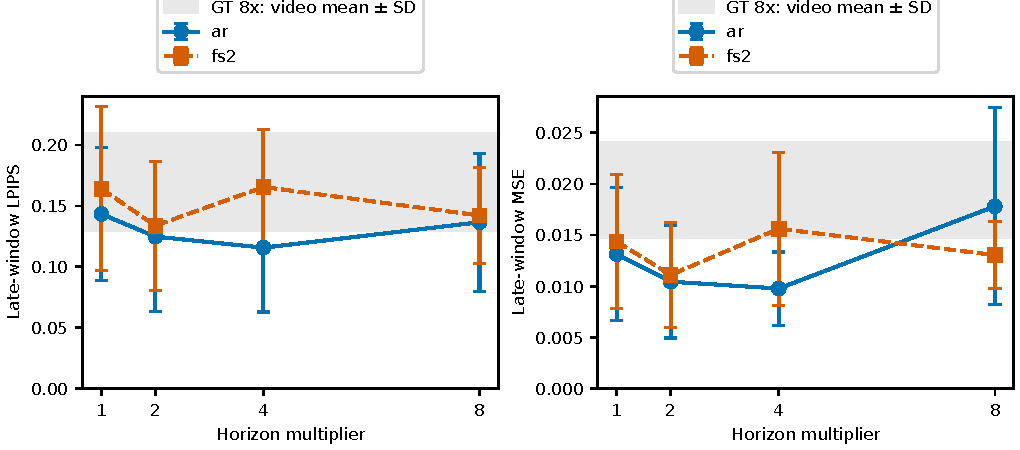
\includegraphics[width=\linewidth]{figures/ablation_summary.pdf}
\caption{Our late-window temporal change versus horizon multiplier. Error bars show standard deviation of seed means when repeats exist, otherwise standard deviation across videos in the single seed. Gray bands show the mean and standard deviation of ground-truth video means from the longest autoregressive run at seed zero, avoiding duplicate references across repeats and schedules.}
\end{figure}}{}

\IfFileExists{tables/ablation_summary.tex}{
\begin{table}[ht]
\centering\begin{tabular}{llrrr}
\toprule
Schedule & Horizon & Late MSE & Late LPIPS & Seconds/video\\
\midrule
ar & 1x & 0.01313 $\pm$ 0.00648 & 0.1433 $\pm$ 0.0543 & 55.00\\
ar & 2x & 0.01044 $\pm$ 0.0055 & 0.1248 $\pm$ 0.0614 & 155.41\\
ar & 4x & 0.009772 $\pm$ 0.00357 & 0.1157 $\pm$ 0.0528 & 358.42\\
ar & 8x & 0.0178 $\pm$ 0.00963 & 0.1366 $\pm$ 0.0566 & 766.33\\
fs2 & 1x & 0.01436 $\pm$ 0.00657 & 0.1641 $\pm$ 0.0675 & 29.77\\
fs2 & 2x & 0.0111 $\pm$ 0.00509 & 0.1337 $\pm$ 0.053 & 81.23\\
fs2 & 4x & 0.01562 $\pm$ 0.00747 & 0.1655 $\pm$ 0.0475 & 183.86\\
fs2 & 8x & 0.01304 $\pm$ 0.00327 & 0.1421 $\pm$ 0.0397 & 387.43\\
\bottomrule
\end{tabular}

\caption{Late-horizon temporal change and end-to-end inference wall time per video. Uncertainty is the standard deviation of seed means when repeated, otherwise the standard deviation across videos. Timing includes process startup and logging.}
\end{table}}{}
\IfFileExists{figures/sanity_curves.pdf}{
\begin{figure}[ht]
\centering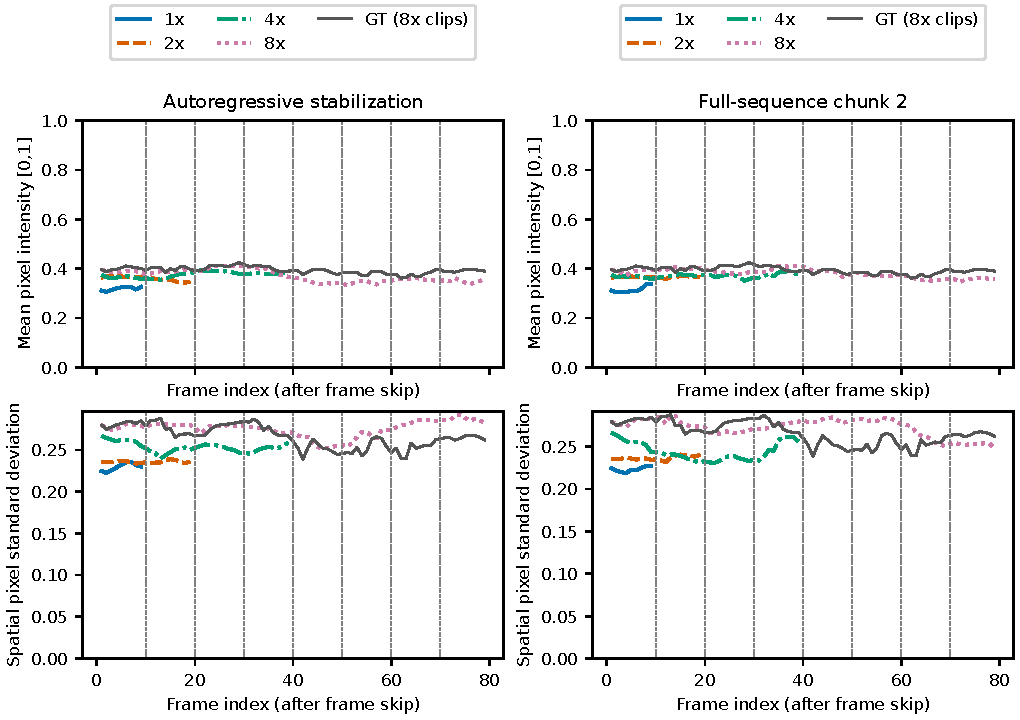
\includegraphics[width=\linewidth]{figures/sanity_curves.pdf}
\caption{Our saturation and collapse checks: mean pixel intensity and spatial pixel standard deviation over time for each sampling schedule and horizon. These complement temporal change, because freezing can produce a near-zero divergence curve without a plausible rollout.}
\end{figure}}{}
\clearpage
\subsection{Guidance-scale sweep}
Guidance scales one through five were evaluated in both mazes at seed zero, with two additional model seeds at default guidance. From scale 1 to 5, medium reward rises from 56.24 to 129.62, success from 55.47\% to 100\%, and censored first-reach steps fall from 436.12 to 226.39. Large reward rises from 109.34 to 170.45 and first-reach steps fall from 518.05 to 338.44; success rises from 72.66\% to 90.63\%, with a small dip at scale 4. Thus stronger guidance generally improves these released-code outcomes, with diminishing reward gains at high scales. Only defaults have repeated model seeds, and all retain fixed environment seed zero. The sweep does not establish a robust optimal scale or a matched advantage over Diffuser.

\IfFileExists{figures/guidance_sweep.pdf}{
\begin{figure}[ht]
\centering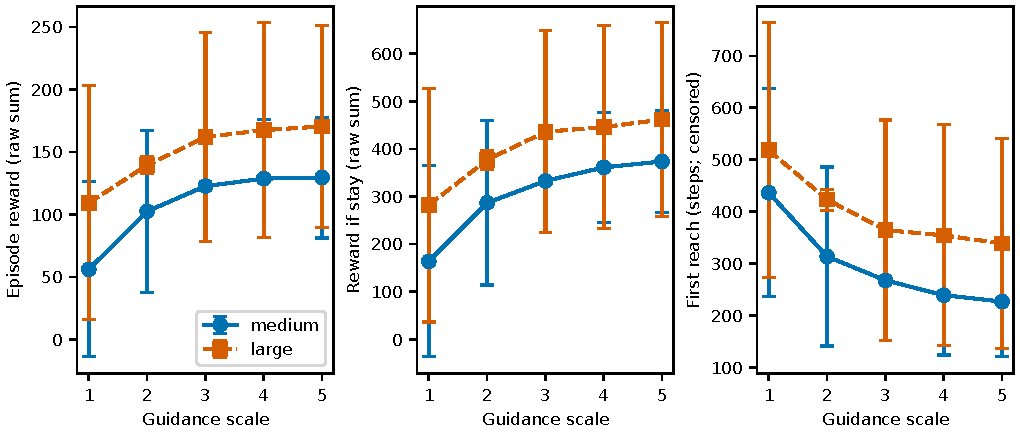
\includegraphics[width=\linewidth]{figures/guidance_sweep.pdf}
\caption{Our guidance-scale ablation: raw episode reward, reward-if-stay and first-reach steps (censored for failures). Error bars show standard deviation of seed means when repeated, otherwise episode standard deviation. These are descriptive uncertainties, not confidence intervals.}
\end{figure}}{}

\clearpage
\paragraph{Planned final-report extension.}
MDF-lite will assign independent noise levels to modalities such as vision, proprioception, force and actions for the team's robot-arm screw-driving task, inspired by Multimodal Diffusion Forcing \cite{huang2026multimodal}. Demonstrations are planned by 2026-11-19 and a trained model by 2026-12-03. This draft contains no implementation or results for that extension.
